\section{System Model}
\label{sec:sysmod}

\begin{figure}
\centering
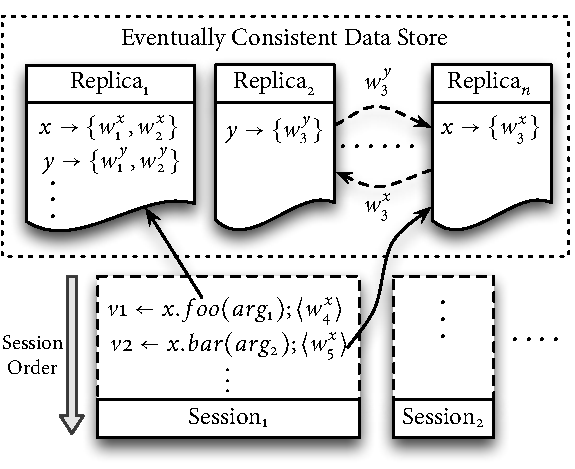
\includegraphics[width=0.8\columnwidth]{Figures/SystemModel}
\caption{\name system model.}
\label{fig:sysmod}
\end{figure}

In this section, we describe the system model and introduce the primitive
relations that our contract language is seeded with. Figure~\ref{fig:sysmod}
presents a schematic diagram of our system model. The distributed store is
composed of a collection of \emph{replicas}, each of which stores a set of
\emph{objects} ($x,y,\ldots$). We assume that every object is replicated at
every replica in the store. The state of an object at any replica is the set of
all updates (\emph{effects}) performed on the object. For example, the state of
$x$ at replica 1 is the set composed of effects $w^x_1$ and $w^x_2$.

Each object is associated with a set of \emph{operations}. The clients interact
with the store by invoking operations on objects. The sequence of operations
invoked by a particular client on the store is called a \emph{session}. The
data store is typically accessed by a large number of clients (and hence
sessions) concurrently. Importantly, the clients are oblivious to which replica
an operation is applied to; the data store may choose to route the operation to
any replica in order to minimize latency, balance load, etc. For example, the
operations \emph{foo} and \emph{bar} invoked by the same session on the same
object, might end up being applied to different replicas because replica 1 (to
which \emph{foo} was applied) might be unreachable when the client invokes
\emph{bar}.

When \emph{foo} is invoked on a object $x$ with arguments \emph{arg}$_1$ at
replica 1, it simply \emph{reduces} over the current set of effects at that
replica on that object ($w^x_1$ and $w^x_2$), produces a result $v1$ that is
sent back to the client, and emits a \emph{single} new effect $w^x_4$ that is
appended to the state of $x$ at replica 1. Thus, every operation is evaluated
over a \emph{snapshot} of the state of the object on which it is invoked. In
this case, the effects $w^x_1$ and $w^x_2$ are \emph{visible} to $w^x_4$,
written logically as $\small \vis{w^x_1}{w^x_4} \wedge \vis{w^x_2}{w^x_4}$,
where $\small \visZ$ is the visibility relation between effects. Visibility is
an irreflexive and asymmetric relation, and only relates effects produced by
operations on the same object. Executing a read-only operation is similar
except that no new effects are produced. The effect added to a particular
replica is asynchronously sent to other replicas, and eventually merged into
all other replicas. Observe that this model does not assume a particular
resolution strategy for concurrent conflicting updates, and instead preserves
\emph{every} update. Update conflicts are resolved when an operation reduces
over the set of effects on an object at a particular replica.

Two effects $w^x_4$ and $w^x_5$ that arise from the same session are said to be
in \emph{session order} (written logically as $\small \so{w^x_4}{w^x_5}$).
Session order is an irreflexive, transitive relation. The effects $w^x_4$ and
$w^x_5$ arising from operations applied to the same object $x$ are said to be
under the \emph{same object} relation, written $\small \sameobj{w^x_4}{w^x_5}$.
Finally, we can associate every effect with the operation that generated the
effect with the help of a relation $\small \operZ$. In the current example,
$\small \oper{w^x_4}{foo}$ and $\small \oper{w^x_5}{bar}$ hold. For simplicity,
we assume all operation names across all object are distinct.

This model admits all the inconsistencies associated with eventual consistency.
The goal of this work is to identify the precise consistency level for each
operation such that application-level constraints are not violated. In the next
section, we will concretely describe the challenges associated with
constructing a consistent bank account on top of an \ecds. Subsequently, we
will illustrate how our contract and specification language, armed with the
primitive relations $\small \visZ$, $\small \soZ$, $\small \sameobjZ$ and
$\small \operZ$, mitigates these challenges.
